\chapter{Revisão da Literatura}

\section{\textit{Learning Management System (LMS)}}
Os \textit{\ac{lms}} – plataformas de apoio à aprendizagem - surgiram para dar apoio à formação a distância online. As plataformas facilitam a disponibilização de recursos em diferentes formatos como texto, vídeo e áudio, apontadores para sites, avisos, interação professor-alunos através de ferramentas de comunicação, ferramentas de apoio à aprendizagem colaborativa e registro das atividades realizadas pelos alunos \cite{rentabilizacao-ens-basico-e-secundario:2007}.


\section{\textit{Gamificação}}
A \textit{gamificação} é uma técnica que envolve dinâmicas, mecanismos e elementos dos \textit{videogames} e os aplica em contextos da vida real. O principal objetivo é engajar as pessoas para que mudem alguns comportamentos, com o propósito de alcançar resultados relacionados a objetivos específicos.


A \textit{gamificação} surge justamente para auxiliar nessa demanda. Em situações em que o engajamento é precário, é possível estabelecer um estímulo extra em contextos que nada têm a ver com jogos, como ambientes corporativos e educacionais.
\cite{gamificacao-corporativa:2017}


Desse modo, pode-se afirmar que a \textit{gamificação} é um processo dedicado ao engajamento de pessoas para que elas produzam mais, independentemente do setor em que estejam inseridas.
\cite{gamificacao-corporativa:2017}


\section{Recompensa}
A recompensa se refere a um prêmio ou retribuição por algo \cite{dicio-recompensa:2009}


Todos gostam de se sentir valorizados por aquilo que produzem. Assim é importante que os gestores se lembrem de implementar alguns mecanismos de recompensas que motivem os colaboradores. \cite{gamificacao-corporativa:2017}


Em uma pesquisa realizada pela \textit{\gls{aberdeen}}, constatou-se que mais da metade dos entrevistados associam a motivação com o reconhecimento por performance. A Figura 1 mostra os fatores motivacionais:

\begin{figure}[htb]
    \centering
	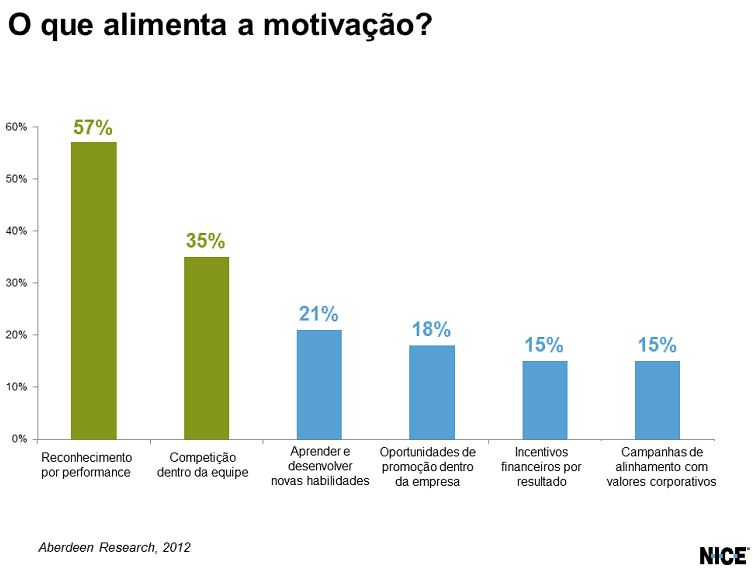
\includegraphics[width=16cm]{imagens/recompensa.jpg}
	\caption{O que alimenta a motivação?}
	\fonte{\cite{grafico-motivacao:2012}}
\end{figure}
\FloatBarrier

\section{Tecnologias}
\subsection{Java}
Java é uma linguagem de programação e plataforma computacional lançada pela primeira vez pela \gls{sun-microsystems} em 1995.


Para criar \textit{applets} e aplicações Java, são necessárias ferramentas de desenvolvimento como o {\ac{jdk}}. O {\ac{jdk}} inclui o \gls{java-runtime-environment}, o \gls{compilador-java} e as \gls{api-java}. É fácil começar a desenvolver programas em Java, tanto para os novos programadores quanto para os experientes \cite{java:2016}.


No projeto Turma de Elite, a linguagem de programação Java será utilizada no \textit{back-end}, apoiado pelo \textit{\gls{framework}} Spring e seus componentes.


\subsection{Spring}
O Spring Framework fornece um modelo abrangente de programação e configuração para aplicativos empresariais modernos baseados em Java - em qualquer tipo de plataforma de implantação.


Um elemento-chave do Spring é o suporte de infraestrutura no nível do aplicativo: o Spring se concentra na "canalização" dos aplicativos corporativos para que as equipes possam se concentrar na lógica de negócios no nível do aplicativo, sem vínculos desnecessários com ambientes de implementação específicos \cite{spring:2021}.

\subsection {Angular}
Angular é uma plataforma de desenvolvimento, construída em 
TypeScript, que inclui:
\begin{itemize}
\item Uma estrutura baseada em componentes para a construção de aplicativos da \textit{\gls{web}} escaláveis;
\item Uma coleção de bibliotecas bem integradas que cobrem uma ampla variedade de recursos, incluindo roteamento, gerenciamento de formulários, e comunicação cliente-servidor;
\item Um conjunto de ferramentas de desenvolvedor capaz de ajudar a desenvolver, construir, testar e atualizar o código \cite{angular:2021}.
\end{itemize}

Será utilizado o Angular como \textit{\gls{framework}} para o \textit{\gls{front-end}} do projeto.

\subsection{MySQL}
Para armazenamento de dados foi escolhido o MySQL. Esse é o banco de dados de código aberto mais popular do mundo. Com seu desempenho comprovado, confiabilidade e facilidade de uso, o MySQL se tornou a principal escolha de banco de dados para aplicativos baseados na web, usados por propriedades da \textit{\gls{web}} de alto perfil, incluindo Facebook, Twitter, YouTube, Yahoo! dentre outros \cite{mysql:2021}.

\subsection{GitHub}
O GitHub oferece um serviço de hospedagem de repositório \gls{git} baseado em nuvem, tornando assim muito mais fácil para que indivíduos e equipes usem o \gls{git} para controle de versão e colaboração.


A interface do GitHub é amigável o suficiente para que até programadores novatos possam utilizar o \gls{git} com facilidade. Sem o GitHub, seria necessário um pouco mais de conhecimento técnico e o uso da linha de comando para o uso do \gls{git} \cite{github:2021}.

\subsection{SVN}
Subversion (\ac{svn}) é um sistema de controle de versão de código aberto. Fundado em 2000 pela CollabNet, \ac{inc}, o projeto e o \textit{\gls{software}} Subversion tiveram um sucesso incrível na última década. O Subversion tem desfrutado e continua a ter ampla adoção tanto na arena do código aberto quanto no mundo corporativo \cite{svn:2021}.


Durante o desenvolvimento, serão utilizados o GitHub e o \ac{svn} para o versionamento de código.

\subsection{Heroku}
Heroku é uma plataforma em nuvem que permite às empresas criar, entregar, monitorar e dimensionar aplicativos, sendo a maneira mais rápida de ir da ideia à \ac{url}.


A plataforma foca incansavelmente em aplicativos e na experiência do desenvolvedor em torno de aplicativos. O Heroku permite que empresas de todos os tamanhos adotem o valor dos aplicativos \cite{heroku:2021}.

\subsection{Travis CI}
Travis \ac{ci} é um serviço de integração onde é possível sincrinizar projetos de código aberto hospedados no GitHub \cite{travis:2021}.

\subsection{Firebase Hosting}
O Firebase Hosting é um recurso de hospedagem de conteúdo da \textit{\gls{web}} de nível de produção para desenvolvedores, sendo possível facilmente implantar apps da \textit{web} de forma rápida e exibir conteúdo estático e dinâmico a uma rede de distribuição de conteúdo (\ac{cdn}) global \cite{hosting:2020}.


O \textit{\gls{back-end}} da aplicação será hospedado no Heroku, utilizando como plataformade \ac{ci}, o Travis. O \textit{\gls{front-end}} da aplicação será hospedado com o serviço Firebase Hosting, do Google.


\subsection{Firebase Authentication}
A maioria dos \textit{\glspl{app}} precisa reconhecer a identidade do usuário. Ter essa informação permite que um \textit{\gls{app}} salve os dados do usuário na nuvem com segurança e forneça a mesma experiência personalizada em todos os dispositivos do usuário \cite{authentication:2020}.


O Firebase Authentication fornece serviços de \textit{\gls{back-end}}, \ac{sdk} fáceis de usar e bibliotecas de \ac{iu} prontas para autenticar usuários no seu aplicativo. Ele oferece suporte à autenticação usando senhas, números de telefone, provedores de identidade federados conhecidos, como Google, Facebook e Twitter, entre outros.


Para dar suporte à autenticação de usuário no sistema, será utilizado o Firebase Authentication.
